
% $Header: /cvsroot/latex-beamer/latex-beamer/solutions/generic-talks/generic-ornate-15min-45min.en.tex,v 1.5 2007/01/28 20:48:23 tantau Exp $

\documentclass[smaller]{beamer}
\mode<presentation>
{
  \usetheme{Singapore}
  \usefonttheme[onlymath]{serif}
  % or ...
 %  \setbeamercovered{transparent}
  % or whatever (possibly just delete it)
}


\usepackage[czech]{babel}
% or whatever
\usepackage[utf8]{inputenc}
% or whatever
%\usepackage{times}
%\usepackage[T1]{fontenc}
% Or whatever. Note that the encoding and the font should match. If T1
% does not look nice, try deleting the line with the fontenc.


\title{PAS12 -- Regresní analýza, Lineární model}

\author{Jan B\v rezina}
\institute % (optional, but mostly needed)
{
  %\inst{2}%
  Technical University of Liberec
}


% If you wish to uncover everything in a step-wise fashion, uncomment
% the following command: 

%\beamerdefaultoverlayspecification{<+->}

% ***************************************** SYMBOLS
\def\div{{\rm div}}
\def\Lapl{\Delta}
\def\grad{\nabla}
\def\supp{{\rm supp}}
\def\dist{{\rm dist}}
%\def\chset{\mathbbm{1}}
\def\chset{1}

\def\Tr{{\rm Tr}}
\def\sgn{{\rm sgn}}
\def\to{\rightarrow}
\def\weakto{\rightharpoonup}
\def\imbed{\hookrightarrow}
\def\cimbed{\subset\subset}
\def\range{{\mathcal R}}
\def\leprox{\lesssim}
\def\argdot{{\hspace{0.18em}\cdot\hspace{0.18em}}}
\def\Distr{{\mathcal D}}
\def\calK{{\mathcal K}}
\def\FromTo{|\rightarrow}
\def\convol{\star}
\def\impl{\Rightarrow}
\DeclareMathOperator*{\esslim}{esslim}
\DeclareMathOperator*{\esssup}{ess\,sup}
\DeclareMathOperator{\ess}{ess}
\DeclareMathOperator{\osc}{osc}
\DeclareMathOperator{\curl}{curl}

%\def\Ess{{\rm ess}}
%\def\Exp{{\rm exp}}
%\def\Implies{\Longrightarrow}
%\def\Equiv{\Longleftrightarrow}
% ****************************************** GENERAL MATH NOTATION
\def\Real{{\rm\bf R}}
\def\Rd{{{\rm\bf R}^{\rm 3}}}
\def\RN{{{\rm\bf R}^N}}
\def\D{{\mathbb D}}
\def\Nnum{{\mathbb N}}
\def\Measures{{\mathcal M}}
\def\d{\,{\rm d}}               % differential
\def\sdodt{\genfrac{}{}{}{1}{\rm d}{{\rm d}t}}
\def\dodt{\genfrac{}{}{}{}{\rm d}{{\rm d}t}}

\def\vc#1{\mathbf{\boldsymbol{#1}}}     % vector
\def\tn#1{{\mathbb{#1}}}    % tensor
\def\abs#1{\lvert#1\rvert}
\def\Abs#1{\bigl\lvert#1\bigr\rvert}
\def\bigabs#1{\bigl\lvert#1\bigr\rvert}
\def\Bigabs#1{\Big\lvert#1\Big\rvert}
\def\ABS#1{\left\lvert#1\right\rvert}
\def\norm#1{\bigl\Vert#1\bigr\Vert} %norm
\def\close#1{\overline{#1}}
\def\inter#1{#1^\circ}
\def\ol#1{\overline{#1}}
\def\ul#1{\underline{#1}}
\def\eqdef{\mathrel{\mathop:}=}     % defining equivalence
\def\where{\,|\,}                    % "where" separator in set's defs
\def\timeD#1{\dot{\overline{{#1}}}}

% ******************************************* USEFULL MACROS
\def\RomanEnum{\renewcommand{\labelenumi}{\rm (\roman{enumi})}}   % enumerate by roman numbers
\def\rf#1{(\ref{#1})}                                             % ref. shortcut
\def\prtl{\partial}                                        % partial deriv.
\def\Names#1{{\scshape #1}}
\def\rem#1{{\parskip=0cm\par!! {\sl\small #1} !!}}

\def\Xint#1{\mathchoice
{\XXint\displaystyle\textstyle{#1}}%
{\XXint\textstyle\scriptstyle{#1}}%
{\XXint\scriptstyle\scriptscriptstyle{#1}}%
{\XXint\scriptscriptstyle\scriptscriptstyle{#1}}%
\!\int}
\def\XXint#1#2#3{{\setbox0=\hbox{$#1{#2#3}{\int}$}
\vcenter{\hbox{$#2#3$}}\kern-.5\wd0}}
\def\ddashint{\Xint=}
\def\dashint{\Xint-}

% ******************************************* DOCUMENT NOTATIONS
% document specific
\def\rh{\varrho}
\def\vl{{\vc{u}}}
\def\th{\vartheta}
\def\vx{\vc{x}}
\def\vX{\vc{X}}
\def\vr{\vc{r}}
\def\veta{\vc{\eta}}
\def\dx{\,\d\vx}
\def\dt{\,\d t}
\def\bulk{\zeta}
\def\cS{\close{S}}
\def\eps{\varepsilon}
\def\phi{\varphi}
\def\Bog{{\mathcal B}}
\def\Riesz{{\mathcal R}}
\def\distr{\mathcal D}
\def\Item{$\bullet$}

\def\MEtst{\mathcal T}
%***************************************************************************
\setbeamercolor{my blue}{fg=blue}
\def\blue#1{{\usebeamercolor[fg]{my blue} #1}}

\setbeamercolor{my green}{fg=green}
\def\green#1{{\usebeamercolor[fg]{my green} #1}}

% color for term definition
\setbeamercolor{my orange}{fg=orange}
\def\df#1{{\usebeamercolor[fg]{my orange} #1}}
\def\xskip{{\vspace{2ex}}}

\def\cz#1{{\small (#1)}}

\def\E{\vc{\mathsf{E}}}

\begin{document}

\begin{frame}
  \titlepage
\end{frame}


\begin{frame}{Motivation example}
 Bending of a beam in dependance of the pressure/force.

 \begin{center}
\begin{tabular}{l|llllll}
pressure $x_i$ & 2 & 4 & 6 & 8 & 10 & 12\\
\hline\\
deformation $Y_i$ & 14 & 35 & 48 & 61 & 80 & 93\\
\end{tabular}
\end{center}

\xskip
\begin{itemize}
  \item We assume, that $x_i$ are exact, without error.
  \item We want to test hypothesis about linear dependency: $y_i= \beta x_i + e_i$.
  \item We assume that $e_i \sim N(0,\sigma^2)$ is independent of $x_i$.
  \item How to get estimate for parameter $\beta$ of the model?
  \item How to compare models $y_i=\beta x_i+e_i$ vs. $y_i=\alpha + \beta x_i +e_i$?
\end{itemize}  
\end{frame}

\begin{frame}{Simplest least squares method}
 Expecting values: $\hat{y}_i = \beta x_i$. We find $\beta$ minimizing
 \[
     S(\beta)= \sum_i (y_i - \hat{y}_i)^2 
 \]
 \dots derivative and solving linear eq. gives estimate $b$
 \[
    b=\frac{\sum_i x_i Y_i}{\sum_i x_i^2}
 \]
 
 We denote $R^2=S(b)$ the \df{residual sum of squares}. The statistics
 \[
    T=\frac{b}{s}\sqrt{\sum_i x_i^2}= b\sqrt{\frac{(n-1)\sum_i x_i^2}{R^2}}, \qquad s^2 = \frac{R^2}{n-1}
 \]
 has distribution $t_{n-1}$. We reject hypothesis $H_0: b=0$, if $T$ is large.
\end{frame}


\begin{frame}{Regression line through origin}
 máme 2 sady dat: $\{X_i\}$, $\{Y_i\}$, $i=1,\dots,n$
 předpokládejme závislost ve tvaru:
 \[
    Y_i = \beta X_i + e_i,
 \]
 kde $e_i$ je NV s rozdělením $N(0,\sigma)$. Rozplyl nezávisí na $i$ !!! 
 
\end{frame}

\begin{frame}{Metoda maximální věrohodnosti}
 Hustota pravděpodobnosti pro náhodný vektor $\vc Y$ je
  \[
   f(Y;b,\sigma) = \frac{1}{(2\pi)^{n/2}\sigma^n} exp\Big\{ -\frac{1}{2\sigma^2} \sum_{i=1}^{n} (Y_i - b X_i)^2 \Big\}
 \]

 Maximalizujeme $f$ vzhledem k $b$, tj. minimalizujeme exponent. 
 Položíme parciální derivace rovné nule:
 \[
    \big(\sum_{i=1}^n X_i^2\big) b = \sum_{i=1}^n X_iY_i 
 \]
 a tedy 
\[ 
   b = \frac{\sum_{i=1}^n X_iY_i}{\sum_{i=1}^n X_i^2}.
\]
... to je bodový odhad parametru $\beta$.
\end{frame}

\begin{frame}{Test o regresním parametru}
Odhad $b$ je lineární kombinace NV $Y_i$ s normálním rozdělením, proto má také normální rozdělení. Určíme jeho parametry:
\[
 E b = \frac{\sum_{i=1}^n X_i E Y_i}{\sum_{i=1}^n X_i^2} = \frac{\sum_{i=1}^n X_i (\beta X_i)}{\sum_{i=1}^n X_i^2} =\beta
\]
\[
 D b = \sum_{i=1}^n \Big(\frac{X_i}{\sum_{i=1}^n X_i^2}\Big)^2 D Y_i = \frac{\sigma^2}{{\sum_{i=1}^n X_i^2}}
\]
Jelikož $\sigma$ neznáme neznáme ani $D b$ jde tedy o odhad sřední hodnoty $\beta$ při neznámém rozptylu:
\[
 T = \frac{b-\beta}{s_b} = \frac{b - \beta}{s} \sqrt{\sum_{i=1}^n X_i^2}
\]
má Studentovo rozdělení $t_{n-1}$, přitom
\[
 s^2 = \frac{R}{n-1} = \frac{\sum (Y_i - b X_i)^2}{n-1}
\]
je reziduální rozptyl, $R$ je reziduální součet čtverců. 
\end{frame}


\begin{frame}{Příklad}
 Průhyb desky v závislosti na tlaku.
\begin{center}
\begin{tabular}{l|llllll}
Tlak $X_i$ & 2 & 4 & 6 & 8 & 10 & 12\\
\hline\\
Průhyb $Y_i$ & 14 & 35 & 48 & 61 & 80 & 93\\
\end{tabular}
\end{center}

\[
  b = 7.857\quad s^2 = 4.7\quad T = 69,041
\]
$t_5(0.975) = 2.571$, zamítáme hypotézu $H0: \beta = 0$. 
%Intevalový odhad je:
%\[
%  b +/- t_5(1-\alpha/2) s / \sqrt{\sum X_i^2} = 7.857 +/- 
%\]

\end{frame}

\begin{frame}{General linear model}
Consider $n$ measurements of a quantity $Y$, that possibly depends on $k$ quantities $X_j$  in linear way:
\[
   \vc{Y} = \sum_{j=1}^k \vc{X_j} \beta_j + \vc{e} = \tn X \vc{\beta} + \vc e
\]
Assume, $\E \vc e = \vc 0$, $var \vc e = \sigma^2 \tn I$. \\
$\sigma^2$ is unknown, $X_{ij}$ are exact.
Determine estimate of $\vc \beta$ by minimization of:
\[
   S(\vc b) = (\vc Y -\tn X\vc b)^T (\vc Y - \tn X\vc b)
\]
Point estimate:
\[
    \vc b = \big( \tn X' \tn X \big)^{-1} \tn X' \vc Y
\]
Residual sum of squares:
\[
    S_e=(\vc Y -\tn X \vc b)^2
\]
Residual variance:
\[
 s^2 = S_e/(n-k) 
\]

\end{frame}

\begin{frame}{Test in general model}
Denote $v_{ij}$ elements of the inverse $\big( \tn X' \tn X \big)^{-1}$, $v_{ii}$ are diagonal entries.
Statistic
\[
  T_i = \frac{b_i - \beta_i}{\sqrt{s^2 v_{ii}}}
\]
have Student distribution $t_{n-k}$.
\end{frame}

\begin{frame}{Application: General line fit}
Model:
\[
  Y_i=\beta_0 + \beta_1 x_i + e_i
\]
Vector notation:
\[
    \vc Y = \tn X\vc \beta, \qquad
    \tn X =
    \begin{pmatrix}
        1 & x_1\\
        \dots \\
        1 & x_n    
    \end{pmatrix}    
\]
\end{frame}


\begin{frame}{Parameter estimates:}
\[
 b_1=\frac{\sum x_i Y_i - n\ol{x}\ol{Y}}
{\sum x_i^2 - n \ol{x}^2}
\]
\[
 b_0=\ol{Y}-b_1\ol{x}
\]
\[
  s^2 =\frac{\sum (Y_i-b_0 - b_1X_i)^2}{n-2}
\]
\end{frame}


\begin{frame}{Anscombe's quartet}
\begin{figure}[h]
 \centering
 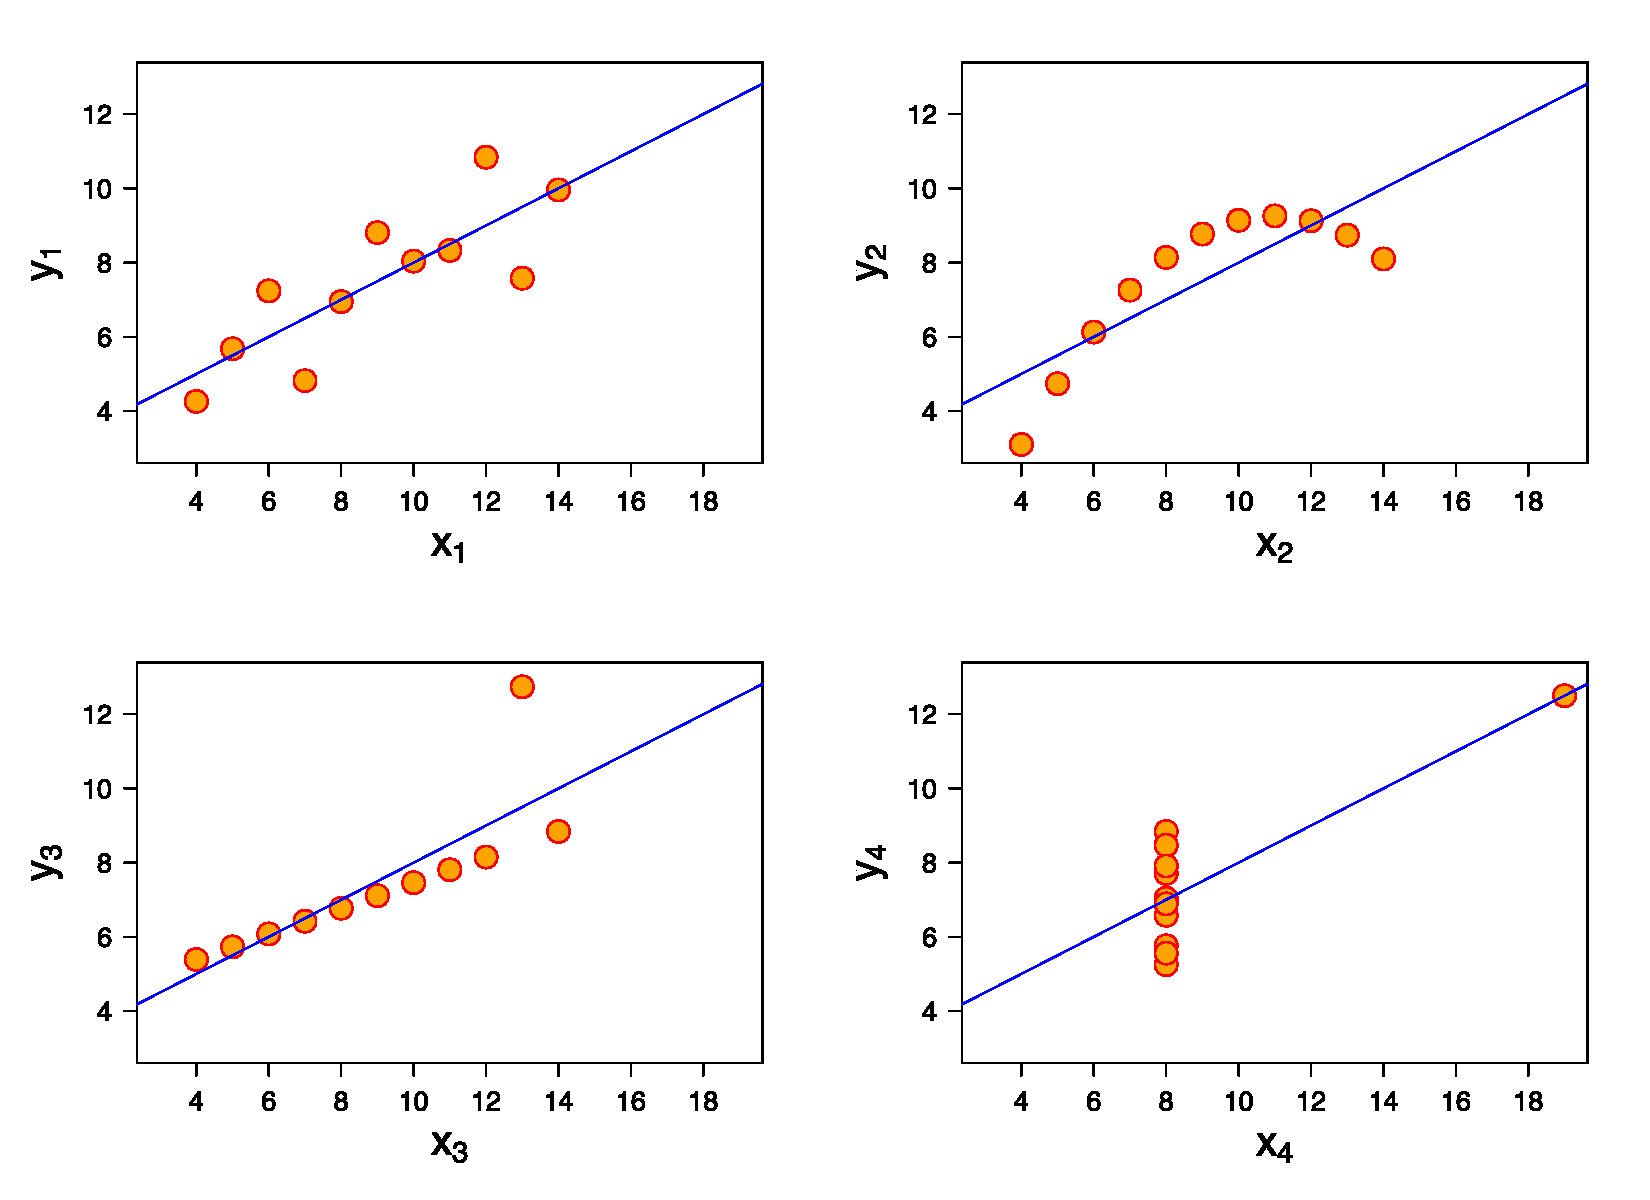
\includegraphics[scale=0.3]{./12_Anscombe's_quartet.pdf}
 % 12_Anscombe's_quartet.svg: 990x720 pixel, 72dpi, 34.92x25.40 cm, bb=0 0 990 720
\end{figure}
\end{frame}

\begin{frame}{Leverage\cz{Pákový efekt}}
Line tangent is weighted average of lines connecting points $(\ol{x},\ol{Y})$  and $(x_i, Y_i)$.
\[
   b_1 =  \sum_i w_i tg \alpha_i
\]

\xskip

\[
    w_i = \frac{(x_i - \ol{x})^2}{\sum_j (x_j - \ol{x})^2}
\]

\xskip

\[
    tg \alpha_i = \frac{Y_i - \ol{Y}}{x_i - \ol{x}}
\]
thus erros in points far from barycenter have significant impact on estimate.

\xskip
Levrage coefficient $h_ii$
\[
    \tn H = \tn X \big( \tn X' \tn X \big)^{-1}\tn X'
\]
\xskip
R software: example(cars)
\end{frame}





\begin{frame}[fragile]{Using R}
\begin{verbatim}
 > d=data.frame( press=seq(2,12,2), def=c(14, 35, 48, 61, 80, 93) )
> plot( def ~ press, data=d)
> model=lm( def ~ press, data=d)
> model
...                                                                                                                                                                                                                                                                               
Coefficients:                                                                                                                                                                                                                                                                  
(Intercept)        press                                                                                                                                                                                                                                                       
     0.8667       7.7571                                                                                                                                                                                                                                                       

> summary(model)                                                                                                                                                                                                                                                               
...                                                                                                                                                                                                                                                                               
Coefficients:                                                                                                                                                                                                                                                                  
            Estimate Std. Error t value Pr(>|t|)                                                                                                                                                                                                                               
(Intercept)   0.8667     2.2180   0.391    0.716                                                                                                                                                                                                                               
press         7.7571     0.2848  27.241 1.08e-05 ***                                                                                                                                                                                                                           
---                                                                                                                                                                                                                                                                            
Residual standard error: 2.382 on 4 degrees of freedom                                                                                                                                                                                                                         
Multiple R-squared: 0.9946,     Adjusted R-squared: 0.9933                                                                                                                                                                                                                     
F-statistic: 742.1 on 1 and 4 DF,  p-value: 1.08e-05   
\end{verbatim}
 
\end{frame}




\end{document}


